%! Author = Len Washington III
%! Date = 3/12/24

% Preamble
\documentclass[lab={3},title={Vowel Lengthening}]{com310lab}

% Packages


% Document
\begin{document}

\maketitle

\begin{overview}
	The duration of vowels varies for a number of reasons: tense vowels are longer than lax ones (\ipa{/i/} vs. \ipa{/I/}); stressed vowels are longer than unstressed ones (e.g., the \ipa{/i/} in \textit{Tina likes BOB vs. TINA likes Bob}); and some vowels are just inherently long.
	For example, Finnish contrasts \ipa{/i/} with \ipa{/i:/}, such that two words can differ only with respect to vowel length alone, and they mean different things, e.g. \ipa{/sika/} `pig' and \ipa{/si:ka/} `whitefish'.
	(The colon indicates `long'.)\\

	Vowel duration in English is measured from the point where vocal fold vibration begins following articulation of a consonant to an abrupt point where a following consonant begins articulation, as with stops, affricates, and fricatives, or to a known acoustic marker signifying a transition to a consonant, as with nasals, liquids and glides.
	Pre-voicing of an initial consonant is not usually included in the vowel duration measure.
	Figure~\ref{fig:vowel-duration} below shows the measurement of vowel duration for the vowel in ``pat''.
	It is reported in milliseconds.

	\begin{figure}[H]
		\centering
		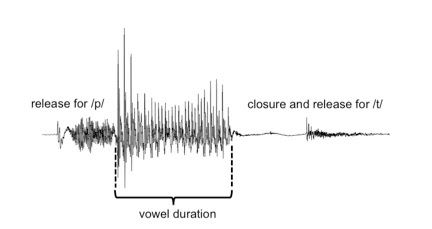
\includegraphics[width=\textwidth]{vowel-duration}
		\caption{Three different VOT values based on the onset of voicing relative to the release of active articulators.}
		\label{fig:vowel-duration}
	\end{figure}~
\end{overview}

\begin{problem}
	Vowel duration varies for reasons other than properties of the vowel itself:
	it can vary in length as a cue to whether a nearby consonant is voiced or voiceless.
	In theory, any vowel lengthening could provide a cue to voicing.
	However, not all consonants will have an effect on vowel length.
	At issue is whether word-initial or -final consonant positions have an effect on vowel length, and whether the effect is uniform across vowels.
\end{problem}

\begin{task}
	Retrieve the set of files containing a set of words in English for this lab.
	There are two speakers, whose recordings are saved in separate files, one labeled \textit{Lab 3 Speaker 1.aiff}, and the other labeled \textit{Lab 3 Speaker 2.aiff}.
	The words and their vowel targets are listed on the following page.

	\begin{table}[H]
		\centering
		\label{tab:vowel-targets}
		\begin{tabular}{*{3}{l   }}
			\textbf{Vowel} & \textbf{Target word} & \textbf{Vowel features}\\
			\ipa{/i/:} & Pete, peed, beet, bead & High front tense\\
			\ipa{/\ae/:} & pat, pad, bat, bad & Low front lax\\
			\ipa{/a/:} & pot, pod, bot, bod & Low front lax\\
			\ipa{/o/:} & tote, toad, dote, Dode & High back tense\\
		\end{tabular}
	\end{table}~

	Use Praat and the guide above to measure vowel duration for all files.
	A demonstration of how to measure vowel length using Praat will be given at the beginning of the lab.
	Then, address the issue raised above: does vowel duration vary as a function of whether the first of last consonant is voiced/voiceless?
	And, is there any variation across vowels?
	Across the two speakers?
	If you are having trouble determining which consonants are voiced or voiceless, use your book, and reference it in your write-up.
\end{task}

\begin{writeup}
	Follow the format for writing up phonetics lab reports and upload your report on Blackboard.\\

	In writing your hypothesis, be sure to state the conditions under which your hypothesis will be supported or refuted.
	You can write something like the following,
	``I predict xxx.
	Evidence in favor of this prediction will be seen if yyy.
	Evidence against this hypothesis will be seen if zzz.''
	Then, in the methods section, clearly explain how the data is collected and analyzed in order to support or refute the hypothesis.
	The results section should be organized solely in the service of addressing whether the hypothesis was supported or not.
	Arrange and summarize the data in order to maximize the reader's understanding of whether to accept or reject the hypothesis, based on the results you obtain.
\end{writeup}

\pagebreak

\labtitle

\begin{topic}
	\\
\end{topic}

\begin{issue}
	\\
\end{issue}

\begin{hypothesis}
	\\
\end{hypothesis}

\begin{method}
	\\
\end{method}

\begin{results}
	\\
\end{results}

\begin{discussion}
	\\
\end{discussion}

\end{document}